\chapter{Scope rules}\label{chap:scope-rules}
This section will be describing scope rules and the environment-store model for the source language. Both are essential for the source language. It is important to know how variables are being stored as well as knowing how the source language is operating with its blocks. 

\section{The environment-store model}\label{sec:es-model}
The environment-store model is important to know how works. The model shows how variables is stored, what variable stored on what location, and with what value. If taking a look on figure \ref{fig:esmodel} one will be seeing the environment-store model. The model shows 3 boxes. 1 box is the environment, 1 is the location and 1 is the store. In the environment is where variables are, the value of these variables has to be stored on a location, which is shown by the arrow, named $env_v$ (variable-environment). On this location the value of the variable can be stored, which is shown with the $sto$ arrow. So if following the model, then the variable $x$ can be found in location 25, which has the value 5 stored. The same principal is valid for $y$ and $z$, however these 2 variables is sharing the same location and which has the same number stored. This also means that if the value in the store is updated, for instance 13 gets changed to 15, then the value in both $y$ and $z$ will change. 
\begin{figure}[H]
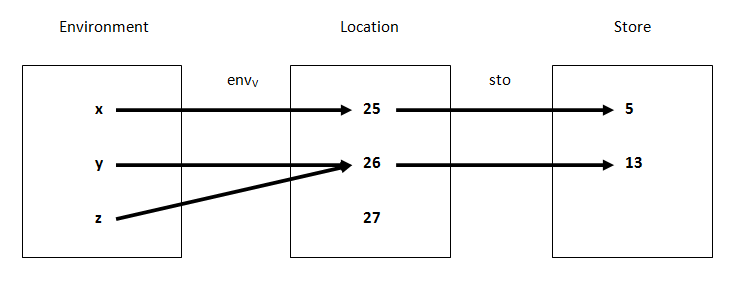
\includegraphics{billeder/environment_store_model.png}
\caption{Environment-store model}
\label{fig:esmodel}
\end{figure}


\section{The scope rules}\label{sec:scope-rules}




\begin{center}
\begin{tabular}{ l l}
\hline
& \\
$[CALL-STAT-STAT_{BSS}]$ & $env'_{v}~[next \rightarrow l], env'_{p}~ \vdash \langle S,sto \rangle \rightarrow sto' \over env_{v}, ~ env_{p} \vdash \langle call~p, sto \rangle \rightarrow sto'$ \\
& where $env_{p}p = (S,env'{v},env'{p})$ \\
& and $l = env_{v}next$ \\
\hline
\end{tabular}
\end{center}







